\documentclass[12pt, legalpaper]{exam}
\usepackage[utf8]{inputenc}
\usepackage[english]{babel}
\usepackage[margin=.8in]{geometry}
\usepackage{amsmath,amssymb}
\usepackage{multicol}
\usepackage{graphicx}
\usepackage{tikz}
\usepackage{lastpage}
\usepackage{tabularx}
\usepackage{hyperref}
\usepackage{tcolorbox}
\newcommand{\course}{Introduction to Optimization}
\newcommand{\term}{Fall 2024}
\newcommand{\examnum}{Report of Programming Task 2}

\usepackage{listings}
\usepackage{xcolor}

\definecolor{codebg}{rgb}{0.95,0.95,0.92}
\definecolor{commentgreen}{rgb}{0,0.6,0}
\definecolor{keywordblue}{rgb}{0,0,0.8}

\lstset{
    backgroundcolor=\color{codebg},
    basicstyle=\ttfamily\footnotesize,
    keywordstyle=\color{keywordblue}\bfseries,
    commentstyle=\color{commentgreen},
    stringstyle=\color{red},
    numbers=left,
    numberstyle=\tiny,
    numbersep=5pt,
    tabsize=4,
    extendedchars=true,
    breaklines=true,
    frame=single,
    showspaces=false,
    showtabs=false,
    showstringspaces=false,
    captionpos=b,
    escapeinside={(*@}{@*)},
}

\begin{document}
\noindent \examnum \, of the  course ''\course'' - \term


\noindent
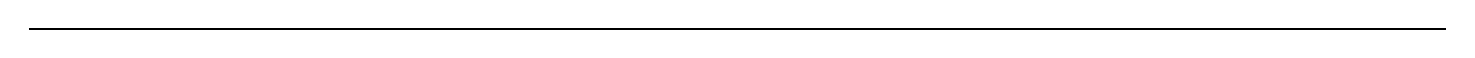
\begin{tikzpicture}
\draw[thick] (0,0) -- (18,0);
\end{tikzpicture}




\vspace{12pt}
\begin{center}
    \textbf{Report 2}
\end{center}
% \noindent \textbf{Requirements}

\vspace{12pt}

\noindent  \textbf{Team information.}

\begin{itemize}
    \item Team leader: Andruwenko Valery 
    \\Grade: 5
    \\ Responsibilities:
    \\Valery coordinated the entire project, distributing tasks to each member to ensure that all assignment stages were addressed efficiently. She also maintained communication with the Teaching Assistant (TA) to keep them informed of the team’s progress and handled the final submission on Moodle. Additionally, Valery prepared a detailed report on each member's contributions, assessing their involvement and performance.
    \item Team member 1: Shariev Marat 
    \\ Grade: 5
    \\Responsibilities:
    \\Marat was primarily responsible for ensuring the correctness and robustness of the working code. He developed several essential functions, including those responsible for finding an initial feasible solution, which was crucial for the program’s operation. Additionally, Marat adjusted the code to make it adaptable for Linear Programming Problems (LPP) with different dimensions, ensuring that the algorithm could handle varying numbers of variables and constraints seamlessly. His contributions were fundamental in making the algorithm reliable and versatile for different problem cases.

    \item Team member 2: Vasilev Ivan
    \\ Grade : 5
    \\Responsibilities:
    \\Ivan focused on implementing the core functionality of the program, specifically writing the Interior-Point algorithm from scratch. His work required meticulous attention to detail, as he had to avoid any built-in functions to meet the assignment’s requirements. Ivan’s task involved developing the algorithm that solved the Linear Programming Problem (LPP), ensuring it adhered to mathematical 

    \item Team member 3: Belyaev Grigorii
    \\ Grade : 5
    \\Responsibilities:
    \\Grigorii was responsible for testing the program. He performed tests on various objective functions and constraints to validate the Interior-Point algorithm’s correctness. His work included checking the algorithm against different scenarios and documenting any bugs or issues encountered, which was essential to ensure the program’s reliability.
\end{itemize}
\vspace{12pt}
\noindent     
\textbf{Link to the product.}
\begin{itemize}
    \item The product is available: \href{https://github.com/GodDamnMan/Optimization_prog_2}{GitHub Repository}
\end{itemize}

\vspace{12pt}

\noindent  \textbf{Programming language.}
\begin{itemize}
    \item Programming language:  Python
\end{itemize}

\vspace{12pt}
\newpage
 
\section*{Test Results}
\section*{Test Case 1}
 
\subsection*{Objective Function}
Maximize \( F(x_1, x_2) = x_1 + x_2 \)
 
\subsection*{Constraints}
\begin{align*}
    2x_1 + 4x_2 &\leq 16, \\
    -x_1 - 3x_2 &\leq -9, \\
    x_1 &\geq 0, \\
    x_2 &\geq 0.
\end{align*}
 
\subsection*{Input}
\begin{verbatim}
Enter the type of the problem (Max/Min): max
NOTE: in input there shouldn't be any slack variables
Enter the coefficients of the objective function: 1 1
Enter amount of the constraints (not assuming x >= 0): 2
Enter the 1st constraint function coefficients: 2 4
Enter the 2nd constraint function coefficients: -1 -3
Enter the right-hand side numbers: 16 -9
\end{verbatim}
 
\subsection*{Expected Output}
\begin{verbatim}
The method is not applicable!
\end{verbatim}
 
\subsection*{Output Evaluation}
The output is correct as the method is not applicable for the given problem setup.
 
\section*{Test Case 2}
 
\subsection*{Objective Function}
Maximize \( F(x_1, x_2, x_3) = 9x_1 + 10x_2 + 16x_3 \)
 
\subsection*{Constraints}
\begin{align*}
    18x_1 + 15x_2 + 12x_3 &\leq 360, \\
    6x_1 + 4x_2 + 8x_3 &\leq 192, \\
    5x_1 + 3x_2 + 3x_3 &\leq 180, \\
    x_1 &\geq 0, \\
    x_2 &\geq 0, \\
    x_3 &\geq 0.
\end{align*}
 
\subsection*{Tableau}
\[
\begin{bmatrix}
    5.00 & 0.00 & 0.00 & 0.22 & 1.67 & 0.00 & 400.00 \\
    x_2 & 1.00 & 1.00 & 0.00 & 0.11 & -0.17 & 0.00 & 8.00 \\
    x_3 & 0.25 & 0.00 & 1.00 & -0.06 & 0.21 & 0.00 & 20.00 \\
    s_3 & 1.25 & 0.00 & 0.00 & -0.17 & -0.12 & 1.00 & 96.00 \\
\end{bmatrix}
\]
 
\subsection*{Basic Variables}
\{ x_2, x_3, s_3 \}
 
\subsection*{All Variables}
\{ x_1, x_2, x_3, s_1, s_2, s_3 \}
 
\subsection*{Input}
\begin{verbatim}
Enter the type of the problem (Max/Min): max
NOTE: in input there shouldn't be any slack variables
Enter the coefficients of the objective function: 9 10 16
Enter amount of the constraints (not assuming x >= 0): 3
Enter the 1st constraint function coefficients: 18 15 12
Enter the 2nd constraint function coefficients: 6 4 8
Enter the 3rd constraint function coefficients: 5 3 3
Enter the right-hand side numbers: 360 192 180
\end{verbatim}
 
\subsection*{Expected Output}
\begin{verbatim}
Optimum is 400.00
x_2 = 8.00
x_3 = 20.00
s_3 = 96.00
\end{verbatim}
 
\subsection*{Output Evaluation}
The output is correct as it satisfies all constraints and provides the maximum profit.
 
\subsection*{Interior Point Iterations}
 
\textbf{Iteration 1:}
\begin{align*}
    \text{For } \lambda = 0.5: & \quad x = [ 3.80, 4.13, 6.02, 157.50, 104.55, 130.57 ] \\
    \text{For } \lambda = 0.9: & \quad x = [ 6.04, 6.63, 10.04, 31.50, 48.98, 99.83 ]
\end{align*}
 
\textbf{Iteration 2:}
\begin{align*}
    \text{For } \lambda = 0.5: & \quad x = [ 4.19, 5.15, 10.71, 78.75, 60.54, 111.45 ] \\
    \text{For } \lambda = 0.9: & \quad x = [ 1.32, 5.51, 19.64, 17.85, 4.90, 97.93 ]
\end{align*}
 
\textbf{Iteration 3:}
\begin{align*}
    \text{For } \lambda = 0.5: & \quad x = [ 3.23, 4.90, 15.34, 44.17, 30.27, 103.11 ] \\
    \text{For } \lambda = 0.9: & \quad x = [ 0.43, 6.40, 20.41, 11.24, 0.49, 97.39 ]
\end{align*}
 
\textbf{Iteration 4:}
\begin{align*}
    \text{For } \lambda = 0.5: & \quad x = [ 2.37, 4.46, 18.10, 33.22, 15.13, 100.46 ] \\
    \text{For } \lambda = 0.9: & \quad x = [ 0.08, 7.85, 19.97, 1.12, 0.34, 96.12 ]
\end{align*}
 
\textbf{Iteration 5 (Last):}
\begin{align*}
    \text{For } \lambda = 0.5: & \quad x = [ 0.00, 8.00, 20.00, 0.00, 0.00, 96.00 ] \\
    \text{For } \lambda = 0.9: & \quad x = [ 0.00, 9.99, 6.76, 0.00, 0.00, 81.82 ]
\end{align*}
 
\textbf{Optimum:}
\begin{align*}
    \text{For } \lambda = 0.5: & \quad \text{Optimum} = 400.0 \\
    \text{For } \lambda = 0.9: & \quad \text{Optimum} = 208.0
\end{align*}
\newpage
\section*{Test Case 3}
 
\subsection*{Objective Function}
Maximize \( F(x_1, x_2, x_3) = x_1 + 3x_2 + 2x_3 \)
 
\subsection*{Constraints}
\begin{align*}
    3x_1 + 2x_2 - x_3 &\leq 9, \\
    2x_1 + 4x_2 + 1x_3 &\leq 10, \\
    x_1 &\geq 0, \\
    x_2 &\geq 0, \\
    x_3 &\geq 0.
\end{align*}
 
 
\[
\begin{array}{|c|c|c|c|c|c|c|}
\hline
    & x_1 & x_2 & x_3 & s_1 & s_2 & \text{Sol} \\
\hline
z   & 3.00 & 5.00 & 0.00 & 0.00 & 2.00 & 20.00 \\
s_1 & 5.00 & 6.00 & 0.00 & 1.00 & 1.00 & 19.00 \\
x_3 & 2.00 & 4.00 & 1.00 & 0.00 & 1.00 & 10.00 \\
\hline
\end{array}
\]
 
\begin{verbatim}
Expected Output:
optimum is 20.00
s1 = 19.00
x3 = 10.00
 
Output Evaluation
The output is correct as it satisfies all constraints and provides the maximum profit.
\end{verbatim}
 
\textbf{Interior Point Iterations:}
\begin{verbatim}
In iteration  1 
        for lambda = 0.5 we have x =  [ 0.98 1.27 1.46 4.98 1.50 ] 
        for lambda = 0.9 we have x =  [ 0.96 1.49 1.83 4.97 0.30 ]
In iteration  2 
        for lambda = 0.5 we have x =  [ 0.88 1.27 2.40 6.22 0.75 ] 
        for lambda = 0.9 we have x =  [ 0.46 0.15 8.36 15.67 0.12 ]
In iteration  3 
        for lambda = 0.5 we have x =  [ 0.67 0.67 5.61 11.26 0.38 ] 
        for lambda = 0.9 we have x =  [ 0.05 0.08 9.50 18.21 0.10 ]
In iteration  4 
        for lambda = 0.5 we have x =  [ 0.47 0.33 7.39 14.30 0.32 ] 
        for lambda = 0.9 we have x =  [ 0.03 0.01 9.85 18.74 0.05 ]
In the last iteration  5 
        for lambda = 0.5 we have x =  [ 0.00 0.00 9.99 18.99 0.00 ] 
        for lambda = 0.9 we have x =  [ 0.00 0.00 10.00 19.00 0.00 ]
 
Optimum:
        for lambda = 0.5 we have: 19.99 
        for lambda = 0.9 we have 20.0
\end{verbatim}
 
\section*{Test Case 4}
\subsection*{Objective Function}
Maximize \( F(x_1, x_2, x_3) = x_1 + x_2 + x_3 + x_4 + x_5 \)
\subsection*{Constraints}
\begin{align*}
    x_1 + x_2 + x_3 + x_4 + x_5 &\leq 1, \\
    2x_1 + 2x_2 + 3x_3 + 4x_4 + 5x_5 &\leq 2, \\
    3x_1 + 3x_2 + 3x_3 + 3x_4 + 3x_5 &\leq 3, \\
    4x_1 + 4x_2 + 4x_3 + 4x_4 + 4x_5 &\leq 4, \\
    5x_1 + 5x_2 + 5x_3 + 5x_4 + 5x_5 &\leq 5, \\
    x_1 &\geq 0, \\
    x_2 &\geq 0, \\
    x_3 &\geq 0, \\
    x_4 &\geq 0, \\
    x_5 &\geq 0.
\end{align*}
 
\subsection*{Input}
\begin{verbatim}
Enter the type of the problem(Max/Min): max
NOTE: in input there shouldn't be any slack variables
Enter the coefficients of the objective function: 1 1 1 1 1
Enter amount of the constraints(not assuming x>=0): 5
Enter the 1 constraint function coefficients: 1 1 1 1 1
Enter the 2 constraint function coefficients: 2 2 2 2 2
Enter the 3 constraint function coefficients: 3 3 3 3 3
Enter the 4 constraint function coefficients: 4 4 4 4 4
Enter the 5 constraint function coefficients: 5 5 5 5 5
Enter the right-hand side numbers: 1 2 3 4 5
Enter the approximation accuracy: 2
\end{verbatim}
 
Expected Output:
\begin{verbatim}
optimum is 1.00
x1 = 1.00
s2 = 0.00
s3 = 0.00
s4 = 0.00
s5 = 0.00
\end{verbatim}
 
Output Evaluation:
The output is correct as it satisfies all constraints and provides the maximum profit.
 
\[
\begin{array}{|c|c|c|c|c|c|c|c|c|c|c|c|}
\hline
    & x_1 & x_2 & x_3 & x_4 & x_5 & s_1 & s_2 & s_3 & s_4 & s_5 & \text{Sol} \\
\hline
z   & 0.00 & 0.00 & 0.00 & 0.00 & 0.00 & 1.00 & 0.00 & 0.00 & 0.00 & 0.00 & 1.00 \\
x_1 & 1.00 & 1.00 & 1.00 & 1.00 & 1.00 & 1.00 & 0.00 & 0.00 & 0.00 & 0.00 & 1.00 \\
s_2 & 0.00 & 0.00 & 0.00 & 0.00 & 0.00 & -2.00 & 1.00 & 0.00 & 0.00 & 0.00 & 0.00 \\
s_3 & 0.00 & 0.00 & 0.00 & 0.00 & 0.00 & -3.00 & 0.00 & 1.00 & 0.00 & 0.00 & 0.00 \\
s_4 & 0.00 & 0.00 & 0.00 & 0.00 & 0.00 & -4.00 & 0.00 & 0.00 & 1.00 & 0.00 & 0.00 \\
s_5 & 0.00 & 0.00 & 0.00 & 0.00 & 0.00 & -5.00 & 0.00 & 0.00 & 0.00 & 1.00 & 0.00 \\
\hline
\end{array}
\]
 
\section*{Interior Point Iterations}
\small
\begin{verbatim}
In iteration  1 
        for lambda = 0.5 we have x =  [ 0.19 0.19 0.19 0.19 0.19 0.05 0.10 0.15 0.20 0.25 ] 
        for lambda = 0.9 we have x =  [ 0.20 0.20 0.20 0.20 0.20 0.01 0.02 0.03 0.04 0.05 ]
In iteration  2 
        for lambda = 0.5 we have x =  [ 0.19 0.19 0.19 0.19 0.19 0.03 0.05 0.08 0.10 0.13 ] 
        for lambda = 0.9 we have x =  [ 0.20 0.20 0.20 0.20 0.20 0.00 0.00 0.00 0.00 0.01 ]
In iteration  3 
        for lambda = 0.5 we have x =  [ 0.20 0.20 0.20 0.20 0.20 0.01 0.03 0.04 0.05 0.06 ] 
        for lambda = 0.9 we have x =  [ 0.20 0.20 0.20 0.20 0.20 0.00 0.00 0.00 0.00 0.00 ]
In iteration  4 
        for lambda = 0.5 we have x =  [ 0.20 0.20 0.20 0.20 0.20 0.01 0.01 0.02 0.03 0.03 ] 
        for lambda = 0.9 we have x =  [ 0.20 0.20 0.20 0.20 0.20 0.00 0.00 0.00 0.00 0.00 ]
In the last iteration  5 
        for lambda = 0.5 we have x =  [ 0.20 0.20 0.20 0.20 0.20 0.00 0.00 0.00 0.00 0.00 ] 
        for lambda = 0.9 we have x =  [ 0.46 0.31 561.70 561.70 5.93 0.00 0.00 0.00 0.00 0.00 ]
 
Optimum:
        for lambda = 0.5 we have: 1.0 
        for lambda = 0.9 we have 1130.08
\end{verbatim}
\normalsize
 
\section*{Test Case 5}
 
\subsection*{Objective Function}
Maximize \( F(x_1, x_2, x_3) = x_1 + 5x_2 + 3x_3 \)
 
\subsection*{Constraints}
\begin{align*}
    x_1 + 2x_2 + x_3 &\leq 3, \\
    2_1 - x_2 &\leq 4, \\
    x_1 &\geq 0, \\
    x_2 &\geq 0, \\
    x_3 &\geq 0.
\end{align*}
 
\[
\begin{array}{|c|c|c|c|c|c|c|}
\hline
    & x_1 & x_2 & x_3 & s_1 & s_2 & \text{Sol} \\
\hline
z   & 2.00 & 1.00 & 0.00 & 3.00 & 0.00 & 9.00 \\
x_3 & 1.00 & 2.00 & 1.00 & 1.00 & 0.00 & 3.00 \\
s_2 & 2.00 & -1.00 & 0.00 & 0.00 & 1.00 & 4.00 \\
\hline
\end{array}
\]
 
\section*{Interior Point Iterations}
\small
\begin{verbatim}
In iteration  1 
        for lambda = 0.5 we have x =  [ 0.41 0.70 1.11 0.09 3.88 ] 
        for lambda = 0.9 we have x =  [ 0.08 0.75 1.35 0.07 4.59 ]
In iteration  2 
        for lambda = 0.5 we have x =  [ 0.20 0.61 1.50 0.07 4.20 ] 
        for lambda = 0.9 we have x =  [ 0.05 0.07 2.77 0.03 3.98 ]
In iteration  3 
        for lambda = 0.5 we have x =  [ 0.10 0.33 2.19 0.05 4.12 ] 
        for lambda = 0.9 we have x =  [ 0.00 0.02 2.94 0.00 4.01 ]
In iteration  4 
        for lambda = 0.5 we have x =  [ 0.07 0.16 2.57 0.04 4.03 ] 
        for lambda = 0.9 we have x =  [ 0.00 0.00 2.99 0.00 4.00 ]
In the last iteration  5 
        for lambda = 0.5 we have x =  [ 0.00 0.00 3.00 0.00 4.00 ] 
        for lambda = 0.9 we have x =  [ 0.00 0.00 3.00 0.00 4.00 ]
 
Optimum:
        for lambda = 0.5 we have: 9.0 
        for lambda = 0.9 we have 9.0
\end{verbatim}
\normalsize
 
 
\subsection*{Input}
\begin{verbatim}
Enter the type of the problem (Max/Min): max
NOTE: in input there shouldn't be any slack variables
Enter the coefficients of the objective function: 9 10 16
Enter amount of the constraints (not assuming x >= 0): 3
Enter the 1st constraint function coefficients: 18 15 12
Enter the 2nd constraint function coefficients: 6 4 8
Enter the 3rd constraint function coefficients: 5 3 3
Enter the right-hand side numbers: 360 192 180
\end{verbatim}
 
\subsection*{Expected Output}
\begin{verbatim}
optimum is 9.00
x3 = 3.00
s2 = 4.00
\end{verbatim}
 
\subsection*{Output Evaluation}
The output is correct as it satisfies all constraints and provides the maximum profit.
 
\vspace{12pt}

\section*{Input Specifications}

The input contains:
\begin{itemize}
    \item \textbf{Problem Type}: A string specifying whether the problem is a maximization (``max'') or minimization (``min'').
    \item \textbf{Objective Function Coefficients}: A vector of floating-point numbers representing the coefficients of the objective function.
    \item \textbf{Number of Constraints}: An integer indicating the number of constraints in the problem.
    \item \textbf{Constraints Matrix}: A matrix where each row represents the coefficients for a single constraint.
    \item \textbf{Right-Hand Side Vector}: A vector of floating-point numbers for the right-hand side of each constraint.
    \item \textbf{Approximation Accuracy}: A positive integer that determines the decimal precision for the solution.
\end{itemize}

\section*{Output Specifications}

The output contains:
\begin{itemize}
    \item \textbf{Error Messages} if input is invalid or the method is not applicable:
    \begin{itemize}
        \item ``ERROR: UNKNOWN TYPE'' if the problem type is not ``max'' or ``min''.
        \item ``ERROR: NO COEFFICIENTS'' if coefficients for the objective function or constraints are missing.
        \item ``ERROR: NOT ENOUGH COEFFICIENTS'' if the constraint matrix or right-hand side vector is incomplete.
        \item ``The problem does not have solution!'' if the problem is unbounded.
        \item ``The Simplex method is not applicable!'' if the Simplex method cannot be applied due to negative values in the right-hand side vector.
        \item ``The method is not applicable!'' if the Interior-Point algorithm cannot solve the problem.
    \end{itemize}
    \item \textbf{Iteration Results}:
    \begin{itemize}
        \item Solution progression over a specified number of iterations (for lambda values of 0.5 and 0.9).
    \end{itemize}
    \item \textbf{Optimal Solution (if applicable)}:
    \begin{itemize}
        \item For each lambda value (0.5 and 0.9), the optimal objective function value in the format:
        \begin{itemize}
            \item ``Optimum with lambda = 0.5 is: [value]''
            \item ``Optimum with lambda = 0.9 is: [value]''
        \end{itemize}
        \item A representation of decision variable values at the optimal solution (e.g., ``x1 = [value]'').
    \end{itemize}
\end{itemize}

\noindent
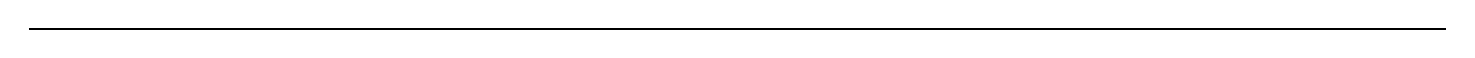
\begin{tikzpicture}
\draw[thick] (0,0) -- (18,0);
\end{tikzpicture}




\vspace{24pt}
\noindent    
\newpage
\textbf{task1}

\begin{lstlisting}[language=Python, caption=Программа на Python, label=lst:python-code]
import math

spacing = 6

class Simplex:
    
    # we define tableu:list (n:int * m:int) - matrix for simplex
    # constrains:list - to check whether tableu ratios are in the scope of them
    # var - ['x1', 'x2', 'x3', 's1', 's2', 's3']
    # basic - ['s1', 's2', 's3']
    def __init__(self, obj_function: list, constrains_matrix: list, right_hand_side_num: list, epsilon:int):
        self.constrains = constrains_matrix
        self.tableu = [[-c for c in obj_function] + [0 for i in range(len(constrains_matrix))] + [0]]
        for i in range(len(constrains_matrix)):
            self.tableu.append([el for el in constrains_matrix[i]] + [1 if i == j else 0 for j in range(len(constrains_matrix))] + [right_hand_side_num[i]])
        
        self.n = len(self.tableu)
        self.m = len(self.tableu[0])
        self.eps = epsilon
        self.basic = [f's{i+1}' for i in range(len(constrains_matrix))]
        self.vars = [f'x{i+1}' for i in range(len(obj_function))] + self.basic
        self.formatting = '{:'+str(self.eps + spacing) + '.' + str(self.eps) + 'f}'
        self.formatting_no_space = '{:'+str(self.eps) + '.' + str(self.eps) + 'f}'
        self.solving = []

    # just simplex 
    def simplex_method(self):
        while True:
            enters = self.solving[0].index(min(self.solving[0]))
            if self.solving[0][enters] >= 0:
                break
            leaves = 0
            l_value = math.inf
            for i in range(1, self.n):
                if self.solving[i][enters] == 0: continue
                temp = self.solving[i][self.m-1]/self.solving[i][enters]
                if (temp < l_value and temp >= 0):
                    leaves = i
                    l_value = temp
            if leaves == 0:
                break

            self.basic[leaves - 1] = self.vars[enters]
            coef = self.solving[leaves][enters]

            for i in range(self.m):
                self.solving[leaves][i] /= coef
        
            for i in range(self.n):
                if i == leaves:
                    continue
                coef = -self.solving[i][enters] / self.solving[leaves][enters]
                for j in range(self.m):
                    self.solving[i][j] += self.solving[leaves][j] * coef

    
    def solve_maximize(self):
        self.solving = self.tableu.copy()
        self.simplex_method()
        self.print_solved()
        return self.solving[0][self.m-1]
        
    
    def solve_minimize(self): 
        self.solving = self.tableu.copy()
        for i in range(self.m):
            self.solving[0][i] *= -1
        self.simplex_method()
        self.print_solved()
        return -self.solving[0][self.m-1]

    
    # function to print initial tableu
    def print_initial(self):
        print("initial tableu:")
        string = '____'
        if ((self.eps + spacing)%2 == 1 or (self.eps + spacing) == 5):
            for j in range (len(self.tableu[0])-1):
                string += "|" + ((self.eps + spacing)//2) * " " + self.vars[j] + ((self.eps + spacing)//2) * " "
            string += "|" + ((self.eps + spacing)//2-1) * " " + "Sol" + (self.eps + spacing)//2 * " " + "|"
            print(string)
        else: 
            for j in range (len(self.tableu[0])-1):
                string += "|" + (self.eps + spacing)//2 * " " + self.vars[j] + ((self.eps + spacing)//2-1) * " "
            string += "|" + ((self.eps + spacing)//2-1) * " " + "Sol" + ((self.eps + spacing)//2-1) * " " + "|"
            print(string)
        k = 0
        for i in self.tableu:
            if(k == 0):
                print(" z  |", end = "")
            else:
                print(self.basic[k-1] + "  |", end = "")
            for j in i:
                print(self.formatting.format(j), end = " |")
            print()
            k+=1
        print()

    # function to print tableu after applying a Simplex method
    def print_solved(self):
        print("optimum is", self.formatting_no_space.format(self.solving[0][self.m-1]))
        for i in range(len(self.basic)):
            print(self.basic[i], "=", self.formatting_no_space.format(self.solving[i+1][self.m-1]))
            
        string = '____'
        if ((self.eps + 4)%2 == 1 or (self.eps + 4) == 5):
            for j in range (len(self.tableu[0])-1):
                string += "|" + ((self.eps + spacing)//2) * " " + self.vars[j] + ((self.eps + spacing)//2) * " "
            string += "|" + ((self.eps + spacing)//2-1) * " " + "Sol" + (self.eps + spacing)//2 * " " + "|"
            print(string)
        else: 
            for j in range (len(self.tableu[0])-1):
                string += "|" + (self.eps + spacing)//2 * " " + self.vars[j] + ((self.eps + spacing)//2-1) * " "
            string += "|" + ((self.eps + spacing)//2-1) * " " + "Sol" + ((self.eps + spacing)//2-1) * " " + "|"
            print(string)

        k = 0
        for i in self.solving:
            if(k == 0):
                print(" z  |", end = "")
            else:
                print(self.basic[k-1] + "  |", end = "")
            for j in i:
                print(self.formatting.format(j), end = " |")
            print()
            k+=1
        print()


def simplex_input():

    type = input("Greetings, this programm will solve your LP problem using Simplex method.\nEnter the type of the problem(Max/Min): ").lower()
    if (type != "max" and type != "min"):
        print("ERROR: UNKNOWN TYPE")
        return
    
    try:
        objective_function = list(map(float, input("Enter the coefficients of the objective function: ").split(" ")))
        if(len(objective_function) == 0):
            print("ERROR: NO COEFFICIENTS")
            return
        
        amount = int(input("Enter amount of the constraints(not assuming x>=0): "))
        if(amount < 1):
            print("ERROR: AMOUNT < 1 ?!")
        constraints = []
        print("Write constraints in format: num num sign\nExample: 3 4 <=")
        for i in range(amount):
            constraint = list(map(float, input(f"Enter the {i+1} constraint function coefficients: ").split(" ")))
            if(len(constraint) == 0):
                print("ERROR: NO COEFFICIENTS")
                return
            constraints.append(constraint)


        right_hand_side = list(map(float, input("Enter the right-hand side numbers: ").split(" ")))
        if(len(right_hand_side) != amount):
            print("ERROR: NOT ENOUGH COEFFICIENTS")
            return
        else:
            for i in right_hand_side:
                if(i < 0):
                    print("The method is not applicable!")
                    return

        accuracy = int(input("Enter the approximation accuracy: "))

        lp = Simplex(objective_function, constraints, right_hand_side, accuracy)
        lp.print_initial()
        if(type == "max"):
            lp.solve_maximize()
        else:
            lp.solve_minimize()
        lp.print_solved()


    except ValueError:
        print("ERROR: NOT A NUMBER")
        return
\end{lstlisting}

\textbf{task2}

\begin{lstlisting}[language=Python, caption=Программа на Python, label=lst:python-code]
import numpy
from numpy.linalg import norm
from task1 import Simplex
from itertools import *
import random
import math

class IteriorPoint:

    def __init__(self, coefs:list, constraints:list, right_hand_side:list, epsilon:int, n:int, isMax:bool):
        self.solution_l1 = None
        self.solution_l2 = None
        self.epsilon = epsilon
        self.right_hand_side = right_hand_side
        self.constraints = constraints
        self.coefs = coefs
        self.alpha1 = 0.5
        self.alpha2 = 0.9
        self.iter_val = 1
        self.n = n
        self.isMax = isMax

    

    def find_initial_solution(self):
        initial_solution = [1 for _ in range(self.n)]

        for i in range(len(self.constraints)):
            initial_solution.append(self.right_hand_side[i] - sum(self.constraints[i][:self.n]))


        dirty_bit = True
        while dirty_bit:
            dirty_bit = False
            for i in range(len(initial_solution)):
                if initial_solution[i] < 0:
                    dirty_bit = True
                    if i < self.n:
                        new_initial_solution = [(initial_solution[j] if j!=i else 0) for j in range(self.n)]
                        
                        for j in range(len(self.constraints)):
                            a = self.constraints[j][:self.n]
                            b = [a[k] * new_initial_solution[k] for k in range(len(a))]
                            new_initial_solution.append(self.right_hand_side[j] - sum(b))
                        initial_solution = new_initial_solution
                        break
                    
                    
                    ind = i - self.n
                    c = -self.constraints[ind][i]
                    grad = [self.constraints[ind][j]/c if j != i else 0  for j in range(len(self.constraints[ind]))] # + [self.right_hand_side[ind]]
                    s = (sum([i**2 for i in grad])) ** 0.5
                    step = 0.1 - initial_solution[i]
                    grad = [j * step / s**2  for j in grad]
                    new_initial_solution = [initial_solution[j] + grad[j] for j in range(self.n)]

                    for j in range(len(self.constraints)):
                        a = self.constraints[j][:self.n]
                        b = [a[k] * new_initial_solution[k] for k in range(len(a))]
                        new_initial_solution.append(self.right_hand_side[j] - sum(b))
                    initial_solution = new_initial_solution
                    break

        self.solution_l1 = initial_solution.copy()
        self.solution_l2 = initial_solution.copy()

    def iterior_point_method(self):
        self.find_initial_solution()
        try:
            while True:
                #calculating previous solution and diagonal matrix for lambda1 and lambda2
                prev_sol_l1 = self.solution_l1
                diagonal_l1 = numpy.diag(self.solution_l1)    

                prev_sol_l2 = self.solution_l2
                diagonal_l2 = numpy.diag(self.solution_l2)

                #calculating matrices for lambda1 and lambda2
                AA_l1 = numpy.dot(self.constraints,diagonal_l1)
                cc_l1 = numpy.dot(diagonal_l1, self.coefs)

                AA_l2 = numpy.dot(self.constraints,diagonal_l2)
                cc_l2 = numpy.dot(diagonal_l2, self.coefs)


                I = numpy.eye(len(self.coefs))


                #components to calculate P for lambda1 and lambda2
                F_l1 = numpy.dot(AA_l1, numpy.transpose(AA_l1))
                FI_l1 = numpy.linalg.inv(F_l1)
                H_l1 = numpy.dot(numpy.transpose(AA_l1), FI_l1)


                F_l2 = numpy.dot(AA_l2, numpy.transpose(AA_l2))
                FI_l2 = numpy.linalg.inv(F_l2)
                H_l2 = numpy.dot(numpy.transpose(AA_l2), FI_l2)

                #calculating P for lambda1 and lambda2
                P_l1 = numpy.subtract(I, numpy.dot(H_l1, AA_l1))
                P_l2 = numpy.subtract(I, numpy.dot(H_l2, AA_l2))

                #calculating cp for lambda1 and lambda2
                cp_l1 = numpy.dot (P_l1, cc_l1)
                cp_l2 = numpy.dot (P_l2, cc_l2)



                nu_l1 = numpy.absolute(numpy.min(cp_l1))
                y_l1 = numpy.add(numpy.ones(len(self.coefs), float), (self.alpha1/nu_l1) * cp_l1)

                nu_l2 = numpy.absolute(numpy.min(cp_l2))
                y_l2 = numpy.add(numpy.ones(len(self.coefs), float), (self.alpha2/nu_l2) * cp_l2)



                yy_l1 = numpy.dot(diagonal_l1, y_l1)
                yy_l2 = numpy.dot(diagonal_l2, y_l2)

                self.solution_l1 = yy_l1
                self.solution_l2 = yy_l2

                if self.iter_val==1 or self.iter_val == 2 or self.iter_val == 3 or self.iter_val == 4:
                    x_l1 = "[ "
                    x_l2 = "[ "
                    for item in self.solution_l1:
                        x_l1 += f'{item:.{self.epsilon}f}' + " "
                    x_l1 += "]"
                    for item in self.solution_l2:
                        x_l2 += f'{item:.{self.epsilon}f}' + " "
                    x_l2 += "]"

                    print("In iteration ", self.iter_val, "\n\tfor lambda = 0.5 we have x = ", x_l1, "\n\tfor lambda = 0.9 we have x = ", x_l2)
                    self.iter_val = self.iter_val + 1

                if norm(numpy.subtract(yy_l1, prev_sol_l1), ord = 2)< 0.00001 or norm(numpy.subtract(yy_l2, prev_sol_l2), ord = 2)< 0.00001:
                    break
        except ValueError:
            x_l1 = "[ "
            x_l2 = "[ "
            for item in self.solution_l1:
                x_l1 += f'{item:.{self.epsilon}f}' + " "
            x_l1 += "]"
            for item in self.solution_l2:
                x_l2 += f'{item:.{self.epsilon}f}' + " "
            x_l2 += "]"
            print ("In the last iteration ", self.iter_val, "\n\tfor lambda = 0.5 we have x = " , x_l1, "\n\tfor lambda = 0.9 we have x = ", x_l2)
            res_l1 = 0
            res_l2 = 0
            for i in range(len(self.coefs)):
                res_l1 += self.coefs[i] * self.solution_l1[i]
                res_l2 += self.coefs[i] * self.solution_l2[i]
            print("\nOptimum:\n\tfor lambda = 0.5 we have:", round(res_l1, self.epsilon), "\n\tfor lambda = 0.9 we have", round(res_l2, self.epsilon))
            raise ValueError
        
        x_l1 = "[ "
        x_l2 = "[ "
        for item in self.solution_l1:
            x_l1 += f'{item:.{self.epsilon}f}' + " "
        x_l1 += "]"
        for item in self.solution_l2:
            x_l2 += f'{item:.{self.epsilon}f}' + " "
        x_l2 += "]"
        print ("In the last iteration ", self.iter_val, "\n\tfor lambda = 0.5 we have x = " , x_l1, "\n\tfor lambda = 0.9 we have x = ", x_l2)
        res_l1 = 0
        res_l2 = 0
        for i in range(len(self.coefs)):
            res_l1 += self.coefs[i] * self.solution_l1[i]
            res_l2 += self.coefs[i] * self.solution_l2[i]
        print("\nOptimum:\n\tfor lambda = 0.5 we have:", round(res_l1, self.epsilon), "\n\tfor lambda = 0.9 we have", round(res_l2, self.epsilon))
            

    def solve_max(self):
        self.iterior_point_method()

    def solve_min(self):
        for item in self.coefs:
            item *= -1
        self.iterior_point_method()

##
# function that will get data from user and check it for some typos, etc.
# and will envoke 2 methods (simplex, iterior-point) if exerything is fine =)
##
def userInput():
    degeneracy_flag = False
    type = input("Greetings, this programm will solve your LP problem using interior-point method.\nEnter the type of the problem(Max/Min): ").lower()
    m = type.index("m")
    type = type[m:m+3]
    if (type != "max" and type != "min"):
        print("ERROR: UNKNOWN TYPE")
        return
    print("NOTE: in input there shouldn't be any slack variables")
    try:
        
        objective_function = input("Enter the coefficients of the objective function: ").split(" ")
        for i in range(objective_function.count("")):
            objective_function.remove("")

        objective_function = list(map(float, objective_function))
        if(len(objective_function) == 0):
            print("ERROR: NO COEFFICIENTS")
            return
        n = len(objective_function)
        

        amount = int(input("Enter amount of the constraints(not assuming x>=0): "))
        if(amount < 1):
            print("ERROR: AMOUNT < 1 ?!")
        constraints = []
        for i in range(amount):
            constraint = input(f"Enter the {i+1} constraint function coefficients: ").split(" ")
            for i in range(constraint.count("")):
                constraint.remove("")
            constraint = list(map(float, constraint))
            if(len(constraint) == 0):
                print("ERROR: NOT ENOUGH COEFFICIENTS")
                return
            constraints.append(constraint)
        

        # Unbounded check
        for j in range(len(constraints[0])):
            f = True
            for i in range(len(constraints)):
                if constraints[i][j] > 0:
                    f = False
                    continue
            if f:
                print("The problem does not have solution!")
                return

        right_hand_side = input("Enter the right-hand side numbers: ").split(" ")
        for i in range(right_hand_side.count("")):
            right_hand_side.remove("")
        right_hand_side = list(map(float, right_hand_side))
        flag_rhs = False
        if(len(right_hand_side) != amount):
            print("ERROR: NOT ENOUGH COEFFICIENTS")
            return
        else:
            for i in right_hand_side:
                if(i < 0):
                    print("The  Simplex method is not applicable!(Input contain negative RHS value)")
                    flag_rhs = True

        accuracy = input("Enter the approximation accuracy: ")

        if accuracy.count('.') == 0: 
            accuracy = int(accuracy)
        else:
            k = 0
            accuracy = float(accuracy)
            while True:
                k += 1
                accuracy *= 10
                if accuracy > 0:
                    break
            accuracy = k

        if(not flag_rhs):
            lp_simplex = Simplex(objective_function, constraints, right_hand_side, accuracy)

        #the following block of code make change of input data for different methods
        for i in range(len(constraints)):
            objective_function.append(0)
            constraint_iter = constraints[i]
            for j in range(len(constraints)):
                if i == j:
                    constraint_iter.append(1)
                else:
                    constraint_iter.append(0)

        # lp_iterior_point = IteriorPoint(objective_function, constraints, right_hand_side, accuracy, n)
        degeneracy_flag = True
        if(type == "max"):
            lp_iterior_point = IteriorPoint(objective_function, constraints, right_hand_side, accuracy, n, True)
            if(not flag_rhs):
                print("===============================================================")
                print ("SIMPLEX")
                lp_simplex.solve_maximize()
            print("===============================================================")
            print ("INTERIOR POINT")
            lp_iterior_point.solve_max()
            print("===============================================================")


        else:
            lp_iterior_point = IteriorPoint(objective_function, constraints, right_hand_side, accuracy, n, False)
            if(not flag_rhs):
                print("===============================================================")
                print ("SIMPLEX")
                lp_simplex.solve_minimize()
            print("===============================================================")
            print ("INTERIOR POINT")
            lp_iterior_point.solve_min()
            print("===============================================================")
        

    except ValueError:
        if not degeneracy_flag: print("ERROR: NOT A NUMBER")
        else: 
            print('DEGENERACY CASE')
            
        return
    

    except numpy.linalg.LinAlgError:
        print("The method is not applicable!")
        return


userInput()


\end{lstlisting}
\end{document}
